% GNUPLOT: LaTeX picture with Postscript
\begingroup
  \makeatletter
  \providecommand\color[2][]{%
    \GenericError{(gnuplot) \space\space\space\@spaces}{%
      Package color not loaded in conjunction with
      terminal option `colourtext'%
    }{See the gnuplot documentation for explanation.%
    }{Either use 'blacktext' in gnuplot or load the package
      color.sty in LaTeX.}%
    \renewcommand\color[2][]{}%
  }%
  \providecommand\includegraphics[2][]{%
    \GenericError{(gnuplot) \space\space\space\@spaces}{%
      Package graphicx or graphics not loaded%
    }{See the gnuplot documentation for explanation.%
    }{The gnuplot epslatex terminal needs graphicx.sty or graphics.sty.}%
    \renewcommand\includegraphics[2][]{}%
  }%
  \providecommand\rotatebox[2]{#2}%
  \@ifundefined{ifGPcolor}{%
    \newif\ifGPcolor
    \GPcolortrue
  }{}%
  \@ifundefined{ifGPblacktext}{%
    \newif\ifGPblacktext
    \GPblacktexttrue
  }{}%
  % define a \g@addto@macro without @ in the name:
  \let\gplgaddtomacro\g@addto@macro
  % define empty templates for all commands taking text:
  \gdef\gplbacktext{}%
  \gdef\gplfronttext{}%
  \makeatother
  \ifGPblacktext
    % no textcolor at all
    \def\colorrgb#1{}%
    \def\colorgray#1{}%
  \else
    % gray or color?
    \ifGPcolor
      \def\colorrgb#1{\color[rgb]{#1}}%
      \def\colorgray#1{\color[gray]{#1}}%
      \expandafter\def\csname LTw\endcsname{\color{white}}%
      \expandafter\def\csname LTb\endcsname{\color{black}}%
      \expandafter\def\csname LTa\endcsname{\color{black}}%
      \expandafter\def\csname LT0\endcsname{\color[rgb]{1,0,0}}%
      \expandafter\def\csname LT1\endcsname{\color[rgb]{0,1,0}}%
      \expandafter\def\csname LT2\endcsname{\color[rgb]{0,0,1}}%
      \expandafter\def\csname LT3\endcsname{\color[rgb]{1,0,1}}%
      \expandafter\def\csname LT4\endcsname{\color[rgb]{0,1,1}}%
      \expandafter\def\csname LT5\endcsname{\color[rgb]{1,1,0}}%
      \expandafter\def\csname LT6\endcsname{\color[rgb]{0,0,0}}%
      \expandafter\def\csname LT7\endcsname{\color[rgb]{1,0.3,0}}%
      \expandafter\def\csname LT8\endcsname{\color[rgb]{0.5,0.5,0.5}}%
    \else
      % gray
      \def\colorrgb#1{\color{black}}%
      \def\colorgray#1{\color[gray]{#1}}%
      \expandafter\def\csname LTw\endcsname{\color{white}}%
      \expandafter\def\csname LTb\endcsname{\color{black}}%
      \expandafter\def\csname LTa\endcsname{\color{black}}%
      \expandafter\def\csname LT0\endcsname{\color{black}}%
      \expandafter\def\csname LT1\endcsname{\color{black}}%
      \expandafter\def\csname LT2\endcsname{\color{black}}%
      \expandafter\def\csname LT3\endcsname{\color{black}}%
      \expandafter\def\csname LT4\endcsname{\color{black}}%
      \expandafter\def\csname LT5\endcsname{\color{black}}%
      \expandafter\def\csname LT6\endcsname{\color{black}}%
      \expandafter\def\csname LT7\endcsname{\color{black}}%
      \expandafter\def\csname LT8\endcsname{\color{black}}%
    \fi
  \fi
  \setlength{\unitlength}{0.0500bp}%
  \begin{picture}(8502.00,6802.00)%
    \gplgaddtomacro\gplbacktext{%
      \csname LTb\endcsname%
      \put(784,1687){\makebox(0,0)[r]{\strut{} 79}}%
      \csname LTb\endcsname%
      \put(784,1960){\makebox(0,0)[r]{\strut{} 79.2}}%
      \csname LTb\endcsname%
      \put(784,2234){\makebox(0,0)[r]{\strut{} 79.4}}%
      \csname LTb\endcsname%
      \put(784,2507){\makebox(0,0)[r]{\strut{} 79.6}}%
      \csname LTb\endcsname%
      \put(784,2781){\makebox(0,0)[r]{\strut{} 79.8}}%
      \csname LTb\endcsname%
      \put(784,3054){\makebox(0,0)[r]{\strut{} 80}}%
      \csname LTb\endcsname%
      \put(784,3328){\makebox(0,0)[r]{\strut{} 80.2}}%
      \csname LTb\endcsname%
      \put(784,3601){\makebox(0,0)[r]{\strut{} 80.4}}%
      \csname LTb\endcsname%
      \put(784,3875){\makebox(0,0)[r]{\strut{} 80.6}}%
      \csname LTb\endcsname%
      \put(784,4148){\makebox(0,0)[r]{\strut{} 80.8}}%
      \csname LTb\endcsname%
      \put(784,4421){\makebox(0,0)[r]{\strut{} 81}}%
      \csname LTb\endcsname%
      \put(784,4695){\makebox(0,0)[r]{\strut{} 81.2}}%
      \csname LTb\endcsname%
      \put(784,4968){\makebox(0,0)[r]{\strut{} 81.4}}%
      \csname LTb\endcsname%
      \put(784,5242){\makebox(0,0)[r]{\strut{} 81.6}}%
      \csname LTb\endcsname%
      \put(784,5515){\makebox(0,0)[r]{\strut{} 81.8}}%
      \csname LTb\endcsname%
      \put(784,5789){\makebox(0,0)[r]{\strut{} 82}}%
      \csname LTb\endcsname%
      \put(784,6062){\makebox(0,0)[r]{\strut{} 82.2}}%
      \csname LTb\endcsname%
      \put(784,6336){\makebox(0,0)[r]{\strut{} 82.4}}%
      \csname LTb\endcsname%
      \put(784,6609){\makebox(0,0)[r]{\strut{} 82.6}}%
      \csname LTb\endcsname%
      \put(880,1408){\rotatebox{-270}{\makebox(0,0)[r]{\strut{}elu}}}%
      \csname LTb\endcsname%
      \put(1223,1408){\rotatebox{-270}{\makebox(0,0)[r]{\strut{}selu}}}%
      \csname LTb\endcsname%
      \put(1565,1408){\rotatebox{-270}{\makebox(0,0)[r]{\strut{}tanh}}}%
      \csname LTb\endcsname%
      \put(1908,1408){\rotatebox{-270}{\makebox(0,0)[r]{\strut{}minsin}}}%
      \csname LTb\endcsname%
      \put(2251,1408){\rotatebox{-270}{\makebox(0,0)[r]{\strut{}maxout-2}}}%
      \csname LTb\endcsname%
      \put(2593,1408){\rotatebox{-270}{\makebox(0,0)[r]{\strut{}penalized\_tanh}}}%
      \csname LTb\endcsname%
      \put(2936,1408){\rotatebox{-270}{\makebox(0,0)[r]{\strut{}maxout-3}}}%
      \csname LTb\endcsname%
      \put(3279,1408){\rotatebox{-270}{\makebox(0,0)[r]{\strut{}sin}}}%
      \csname LTb\endcsname%
      \put(3621,1408){\rotatebox{-270}{\makebox(0,0)[r]{\strut{}maxout-4}}}%
      \csname LTb\endcsname%
      \put(3964,1408){\rotatebox{-270}{\makebox(0,0)[r]{\strut{}prelu}}}%
      \csname LTb\endcsname%
      \put(4307,1408){\rotatebox{-270}{\makebox(0,0)[r]{\strut{}leakyrelu-0.3}}}%
      \csname LTb\endcsname%
      \put(4649,1408){\rotatebox{-270}{\makebox(0,0)[r]{\strut{}linear}}}%
      \csname LTb\endcsname%
      \put(4992,1408){\rotatebox{-270}{\makebox(0,0)[r]{\strut{}maxtanh}}}%
      \csname LTb\endcsname%
      \put(5334,1408){\rotatebox{-270}{\makebox(0,0)[r]{\strut{}leakyrelu-0.01}}}%
      \csname LTb\endcsname%
      \put(5677,1408){\rotatebox{-270}{\makebox(0,0)[r]{\strut{}relu}}}%
      \csname LTb\endcsname%
      \put(6020,1408){\rotatebox{-270}{\makebox(0,0)[r]{\strut{}tanhrev}}}%
      \csname LTb\endcsname%
      \put(6362,1408){\rotatebox{-270}{\makebox(0,0)[r]{\strut{}swish}}}%
      \csname LTb\endcsname%
      \put(6705,1408){\rotatebox{-270}{\makebox(0,0)[r]{\strut{}cosper}}}%
      \csname LTb\endcsname%
      \put(7048,1408){\rotatebox{-270}{\makebox(0,0)[r]{\strut{}sigmoid}}}%
      \csname LTb\endcsname%
      \put(7390,1408){\rotatebox{-270}{\makebox(0,0)[r]{\strut{}maxsig}}}%
      \csname LTb\endcsname%
      \put(7733,1408){\rotatebox{-270}{\makebox(0,0)[r]{\strut{}cube}}}%
      \put(7829,2171){\makebox(0,0)[l]{\strut{} 45}}%
      \put(7829,3059){\makebox(0,0)[l]{\strut{} 50}}%
      \put(7829,3946){\makebox(0,0)[l]{\strut{} 55}}%
      \put(7829,4834){\makebox(0,0)[l]{\strut{} 60}}%
      \put(7829,5721){\makebox(0,0)[l]{\strut{} 65}}%
      \put(7829,6609){\makebox(0,0)[l]{\strut{} 70}}%
      \csname LTb\endcsname%
      \put(128,4056){\rotatebox{-270}{\makebox(0,0){\strut{}Score}}}%
    }%
    \gplgaddtomacro\gplfronttext{%
      \csname LTb\endcsname%
      \put(6998,1807){\makebox(0,0)[r]{\strut{}Best}}%
      \csname LTb\endcsname%
      \put(6998,1647){\makebox(0,0)[r]{\strut{}Avg}}%
    }%
    \gplbacktext
    \put(0,0){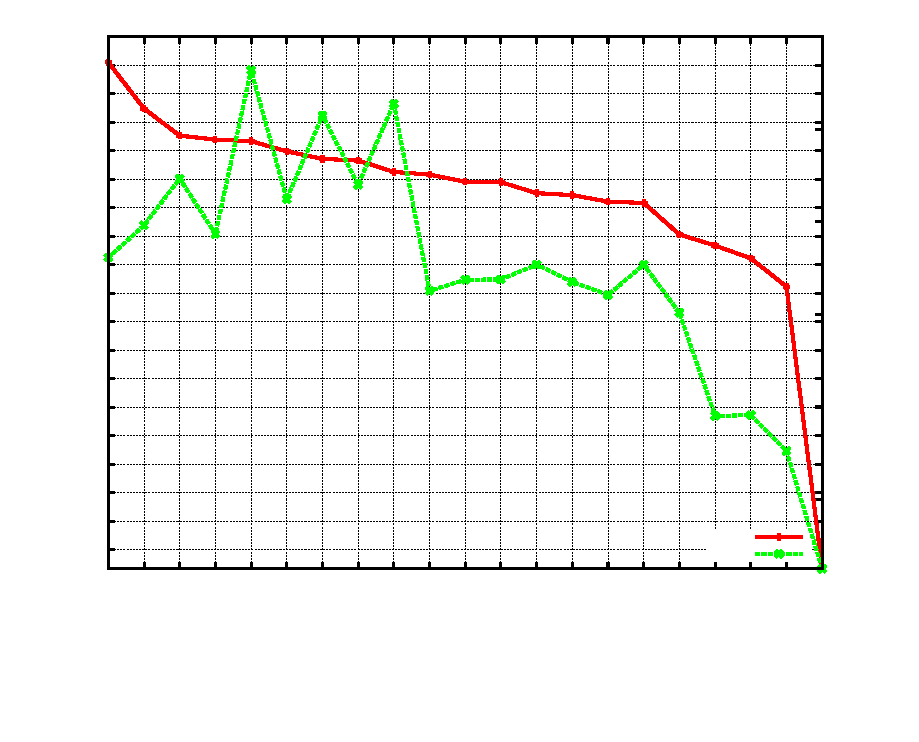
\includegraphics{plots/doc2}}%
    \gplfronttext
  \end{picture}%
\endgroup
